\section{Netzwerkanalyse}

\begin{multicols}{2}
\subsection{Serieschaltung von Widerständen}
$ R_{ges} = \sum\limits_{k=1}^{n}{R_k} $ \\

\subsection{Parallelschaltung von Widerständen}
$ \frac{1}{R_{ges}} = \sum\limits_{k=1}^{n}\frac{1}{R_k}\ \ \ \rightarrow R_{ges_2} = \frac{R_1 \cdot R_2}{R_1 + R_2} $ \\
\begin{multicols}{2}
\subsection{Spannungsteiler}
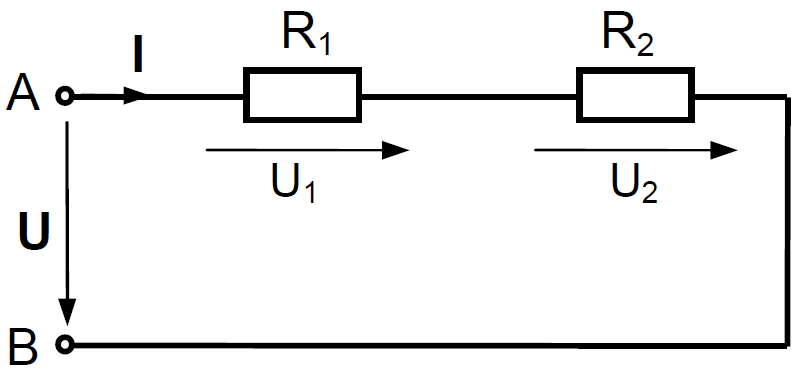
\includegraphics[width=0.20\textwidth]{pics/spannungsteiler}\\
$ U_1 = U \cdot \frac{R_1}{R_1 + R_2}$ \\
$ U_2 = U \cdot \frac{R_2}{R_1 + R_2}$ \\

\subsection{Stromteiler}
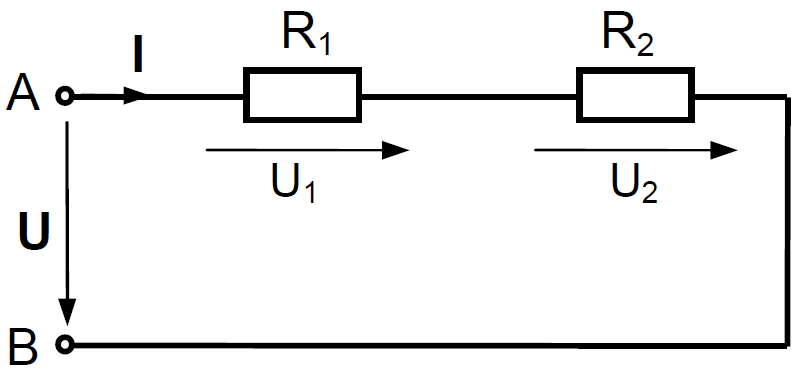
\includegraphics[width=0.15\textwidth]{pics/stromteiler}\\
$ I_1 = I \cdot \frac{R_2}{R_1 + R_2}$ \\
$ I_2 = I \cdot \frac{R_1}{R_1 + R_2}$ \\
\end{multicols}
\end{multicols}

\subsection{Kirchhof}
\begin{multicols}{4}
{\centering
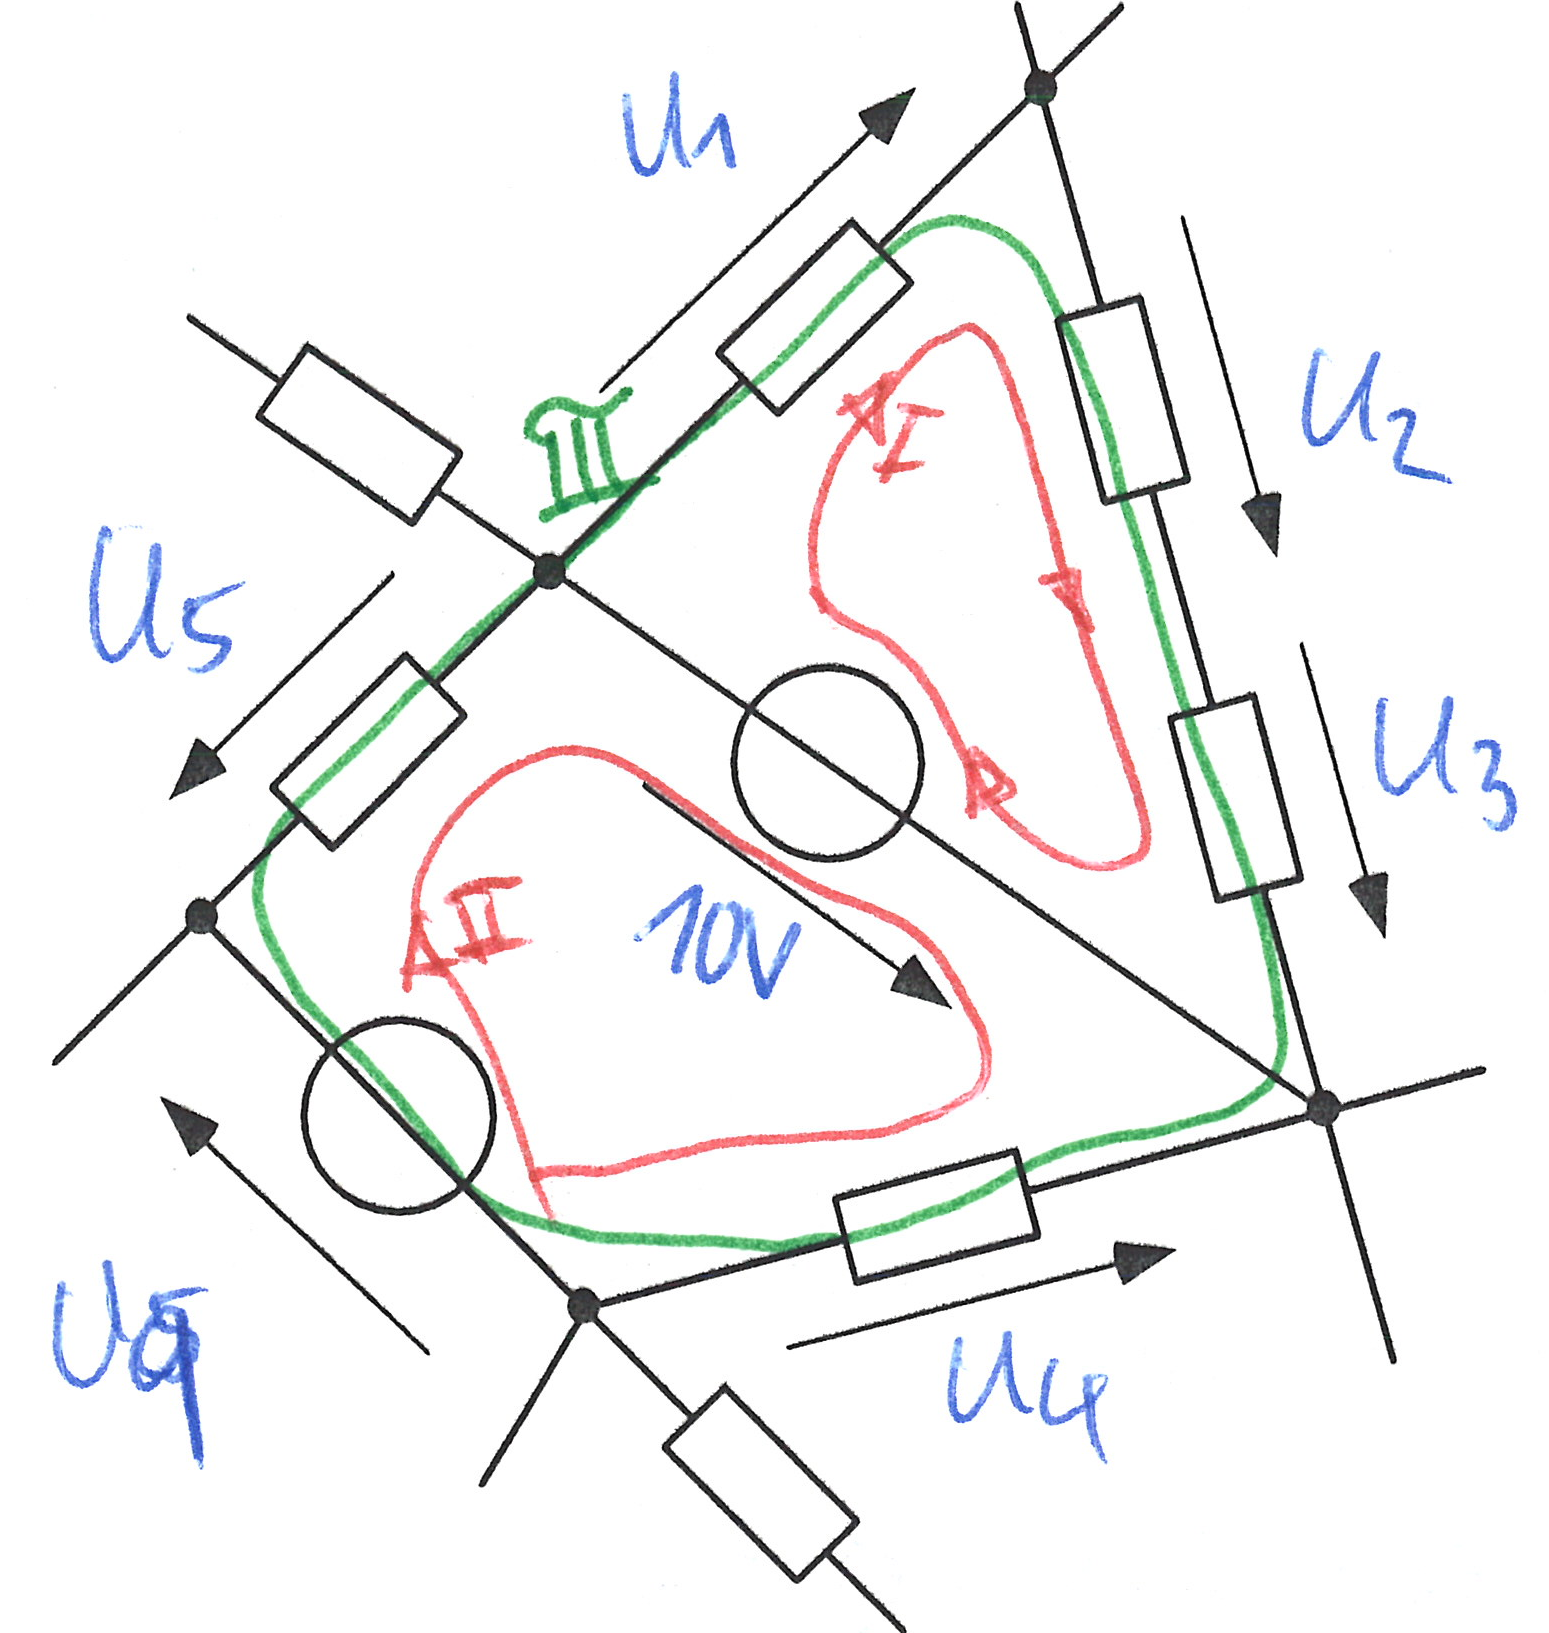
\includegraphics[width=0.12 \textwidth]{pics/kirchhof/masche}\\}
\textbf{2. Kirchhofschesgesetz}\\
Maschensatz: Summe aller Spannungen =0.\\
	$U_1+U_2+U_3-10V=0$
	$10V-U_4+U_q-U_5=0$
	$U_1+U_2+U_3-U_4+U_q-U_5=0$\\
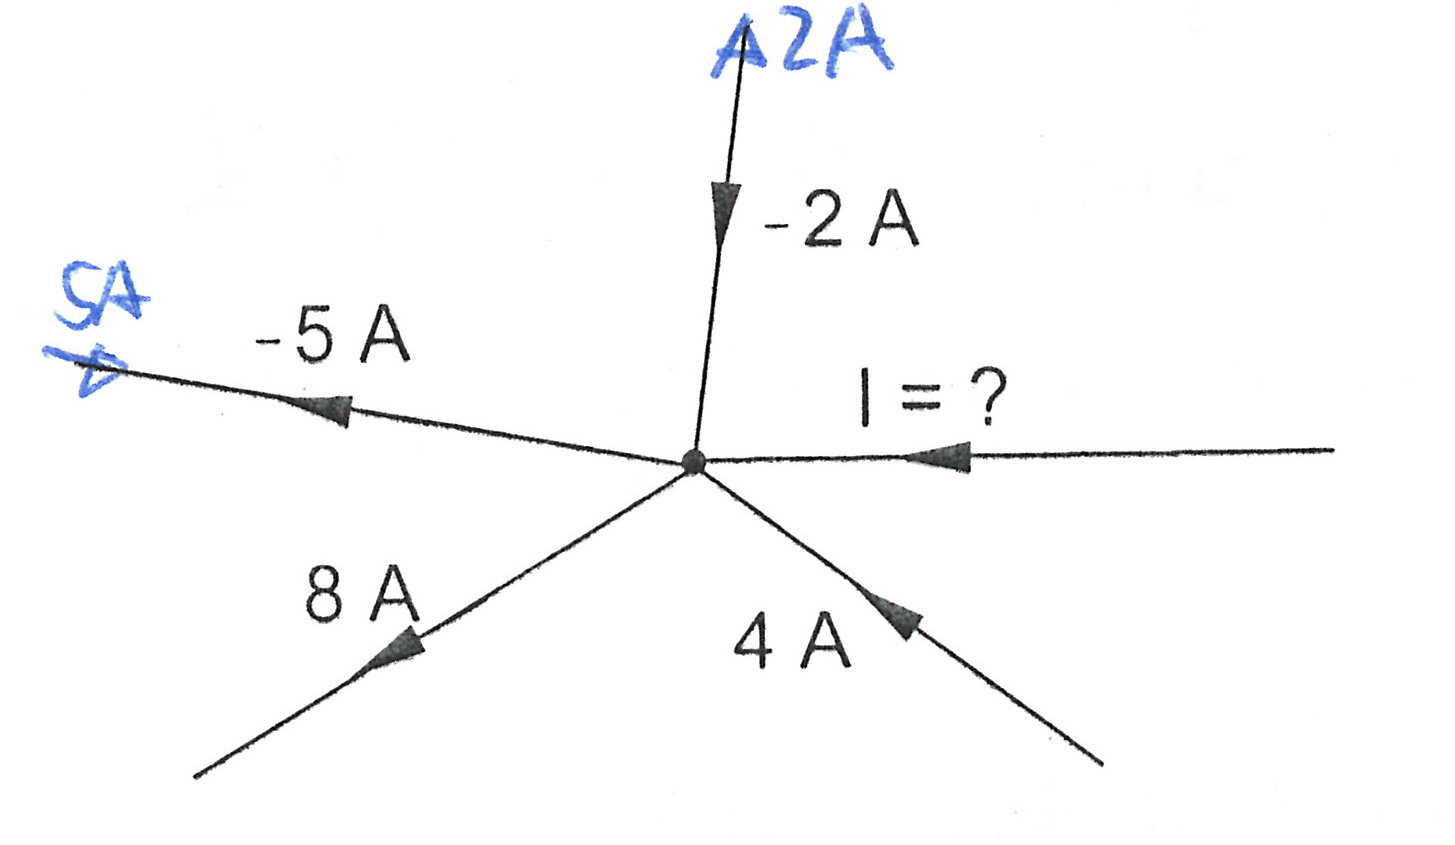
\includegraphics[width=0.24\textwidth]{pics/kirchhof/knoten}\\
\textbf{1. Kirchhofschesgesetz}\\
Konotensatz: Summer aller Str"ome = 0, zufliessende Ströme positiv abfliessende Ströme negativ.\\
$4A-8A+5A-2A+I=0A$\\
\end{multicols}

\subsection{Stern Dreieck Umwandlung}
\begin{multicols}{3}
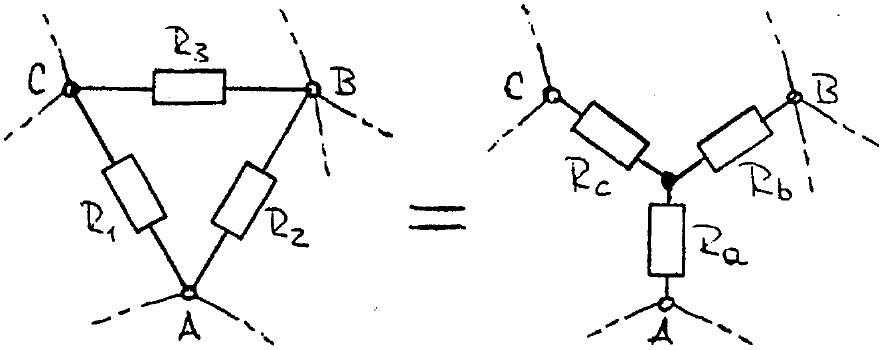
\includegraphics[width=0.3\textwidth]{pics/stern-dreieck}
\subsubsection{$ \triangle \rightarrow $ Y}
$ R_0 = R_1 + R_2 + R_3 $ \\
$ R_a = \frac{R_1R_2}{R_0} = \frac{R_1R_2}{R_1 + R_2 + R_3} $ \\[1pt]
$ R_b = \frac{R_2R_3}{R_0} = \frac{R_2R_3}{R_1 + R_2 + R_3} $ \\[1pt]
$ R_c = \frac{R_1R_3}{R_0} = \frac{R_1R_3}{R_1 + R_2 + R_3} $ \\
\subsubsection{Y $ \rightarrow \triangle $}
$ G_0 = G_a + G_b + G_c = \frac{1}{R_a} + \frac{1}{R_b} + \frac{1}{R_c} $ \\
$ R_1 = R_aR_cG_0 = R_aR_c(\frac{1}{R_a} + \frac{1}{R_b} + \frac{1}{R_c}) $ \\
$ R_2 = R_aR_bG_0 = R_aR_b(\frac{1}{R_a} + \frac{1}{R_b} + \frac{1}{R_c}) $ \\
$ R_3 = R_bR_cG_0 = R_bR_c(\frac{1}{R_a} + \frac{1}{R_b} + \frac{1}{R_c}) $ \\
\end{multicols}

\subsection{Begriffe, Definition}
\begin{tabular}{lll}
Knoten & (Verbindungspunkte) & Anzahl: k \\
Zweige & (Verbindungen zwischen Knoten) & Anzahl: z \\
Vollständiger Baum & Nicht geschlossener Linienzug, verbindet sämtliche Knoten& \\
Baumzweige ("Aste) & &  Anzahl: k-1\\
Verbindungszweige (Sehnen) & Alle Zweige, die nicht zum Baum gehören & Anzahl: z-(k-1)=z-k+1\\
Kreis & Geschlossene Folge von Zweigen, enthält keinen Knoten zweimal & \\
Masche & Kreis, der entweder innerhalb oder ausserhalb keine Zweige enthält & \\
Planares Netzwerk & Netzwerk ohne Kreuzung von Zweigen & \\
\end{tabular}

\subsection{Aspekte zur Wahl der Methode}
\begin{tabular}{lll}
	\multicolumn{3}{l}{Die \textit{Art der gegebenen Quellen} ist wohl die wichtigste Entscheidungsgrundlage:}\\
	&Kreisstrommethode: &Spannungsquellen\\
	&Knotenpotentialmethode: &Stromquellen\\
	\multicolumn{3}{l}{Die \textit{Anzahl Gleichungen} kann auch entscheidend sein:}\\
	&Kreisstrommethode: &$z-k+1-$ Anzahl idealer Stromquellen\\
	&Knotenpotentialmethode: &$k-1-$ Anzahl idealer Spannungsquellen\\
	\multicolumn{3}{l}{Ein kleines Argument dürften die \textit{gesuchten Grössen} sein (Umformung durch $U=R \cdot I$):}\\
	&Kreisstrommethode: &(Sehnen-) Ströme\\
	&Knotenpotentialmethode: &(Knoten-) Spannungen
\end{tabular}

\subsection{Wahl von Kreisen}
\begin{itemize}
\item \textbf{Allgemein}
Beim Einzeichnen eines Kreises einen Zweig davon markieren (abstreichen und nummerieren). Diesen Zweig bei den weiteren Kreisen nicht mehr verwenden. Anzahl Kreise: $m = z-k+1$\\[-5pt]
\item \textbf{Kreisstrommethode}
Man zeichnet einen vollständigen Baum. Jeder Kreis soll eine andere Sehne (und nur diese) enthalten $\rightarrow$ "`Basiskreis"'\\[-5pt]
\item \textbf{Maschenstrommethode}
Man wählt als Kreise lauter Maschen (z.B. alle inneren, oder äussere und eine innere weniger). Voraussetzung: Netzwerk planar\\[-5pt]
\end{itemize}

\subsection{Maschen- und Kreisstrommethode}
Der Unterschied zwischen diesen beiden Analysemethoden ist, dass die Kreisstrommethode allgemeiner ist. Bei der Maschenmethode wird jede Masche als Kreis behandelt, bei der Kreisstrommethode können Kreise auch als "`Nicht-Maschen"' angesehen werden.
Besonders bei der Maschenstrommethode kann die Matrix durch Einzeichngen der Bezugspfeile in dieselbe Richtung enorm vereinfacht werden$\rightarrow$Elemente ausserhalb diagonale werden negativ.
\begin{figure}[hct]
  \begin{minipage}[t]{8 cm} %BASTEL!!
	  \centering
	  Maschenstrommethode:\\
	  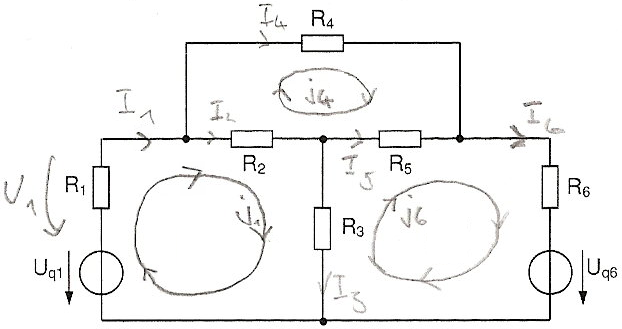
\includegraphics[width=7cm]{pics/dcnet/maschenmethode}
	 \end{minipage}
	 \begin{minipage}[t]{10 cm}
	  \centering
	  Kreisstrommethode:\\
	  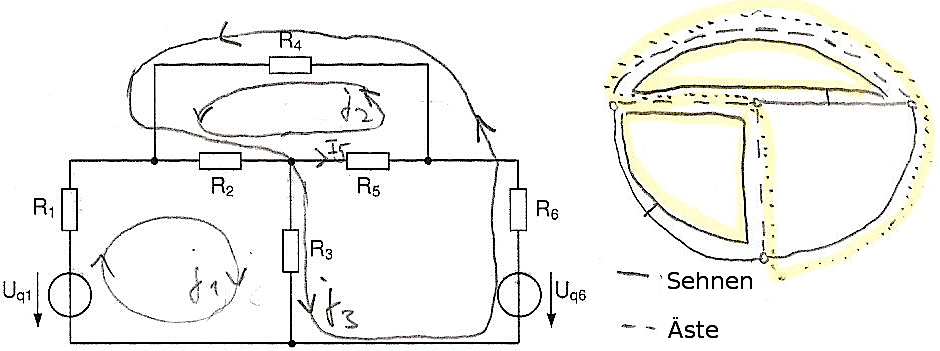
\includegraphics[width=10cm]{pics/dcnet/kreisstrommethode} 
  \end{minipage}
\end{figure}

\textbf{Quellen:} Spannungspfeil gegen Bezugsrichtung (Strom in Bezugsrichtung) des Kreises $\rightarrow$ Spannung auf rechter Seite positiv.\\

Passende Matrix zur Maschenstrommethode:

$\left[\begin{array}{ccc}
	+R_1+R_2+R_3 &\hervor{-}R_2 &\hervor{-}R_3  \\
	\hervor{-}R_2 &+R_2+R_4+R_5
	&\hervor{-}R_5\\ 
	\hervor{-}R_3 &\hervor{-}R_5 &+R_3+R_5+R_6
	\end{array}\right] \bullet 
	\left[\begin{array}{l}j_1\\j_4\\j_6\end{array}\right] = 
	\left[\begin{array}{c}\hervor{+}U_{q1}\\0\\
	\hervor{-}U_{q6}
\end{array}\right]$\\

Passende Matrix zur Kreisstrommethode:

$\left[\begin{array}{ccc}
	+R_1+R_2+R_3 &\hervor{+}R_2 &\hervor{+}R_2+R_3\\
	\hervor{+}R_2 &+R_2+R_4+R_5
	&\hervor{+}R_2+R_4\\ 
	\hervor{+}R_2+R_3 &\hervor{+}R_2+R_4 &+R_2+R_3+R_4+R_6
	\end{array}\right] \bullet 
	\left[\begin{array}{l}j_1\\j_2\\j_3\end{array}\right] = 
	\left[\begin{array}{c}\hervor{+}U_{q1}\\0\\
	\hervor{+}U_{q6}
\end{array}\right]$\\

Der Vorteil der Kreisstrommethode gegenüber der Maschenstrommethode ist der,dass ein gewünschter Strom direkt aus der Gleichung ausgerechnet werden kann. In diesem Beispiel wäre bspw. $I_5 = j_2\rightarrow$ Muss in Sehne liegen.

\subsection{Knotenpotentialmethode}
\begin{figure}[hct]
  \begin{minipage}[lt]{7 cm}
    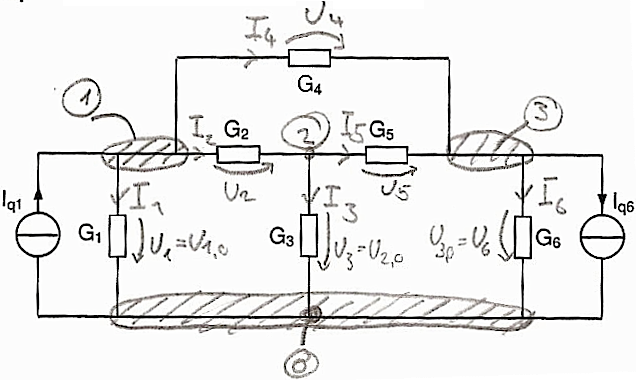
\includegraphics[width=7cm]{pics/dcnet/knotenpotentialmethode} 
  \end{minipage}
  \begin{minipage}[rt]{9.35 cm} %BASTEL!!
  Bei dieser Methode wird immer mit \textit{Leitwerten} $G$  und (idealen) \textit{Stromquellen}
gerechnet. Siehe auch S. 33 im Formelbuch.
  \end{minipage}
\end{figure}

\textbf{Quellen:} Strom in Knoten hinein $\rightarrow$ Strom auf rechter Seite positiv.\\

$\left[\begin{array}{ccc}
+G_1+G_2+G_4 &\hervor{-}G_2 &\hervor{-}G_4\\
\hervor{-}G_2 &+G_2+G_3+G_5
&\hervor{-}G_5\\ 
\hervor{-}G_4 &\hervor{-}G_5 &+G_4+G_5+G_6
\end{array}\right] \bullet 
\left[\begin{array}{l}U_1\\U_2\\U_3\end{array}\right] = 
\left[\begin{array}{c}\hervor{+}I_{q1}\\0\\
\hervor{-}I_{q6}\end{array}\right]$

Nebenelemente(nicht auf diagonale) $\rightarrow$ Leitwerte zwischen jeweiligen Knoten $\rightarrow$ Falls anderer Knoten dazwischen $\rightarrow$ $G$ = 0

\subsection{Behandlung idealer Quellen}
\subsubsection{Kreisstrom- bzw. Maschenstrommethode:}
\begin{itemize}
	\item \textbf{Spannungsquellen} (lineare oder ideale) können ohne weiteres in die Netzwerkgleichungen einbezogen werden. Die Quellenspannung erscheint "`rechts"' des Gleichheitszeichens als sogenannte Störfunktion.
	\item \textbf{Lineare Stromquellen} ($G_{i} \not = 0$) werden in Spannungsquellen umgewandelt
	\item \textbf{Ideale Stromquellen} erforden eine Sonderbehandlung\\ $\rightarrow$ Quellenströme gleich als Kreisströme benutzen(Quellen in Sehnen von Basiskreisen legen!)\\$\rightarrow$ Falls dies nicht möglich ist $\rightarrow$ Quellen verschieben und in Spannungsquellen umwandeln
\end{itemize}
\emph{Pro ideale Stromquelle vermindert sich die Zahl der Netzwerkgleichungen und die Zahl der Unbekannten um eins!}

\subsubsection{Knotenpotentialmethode:}
\begin{itemize}
	\item \textbf{Stromquellen}(lineare oder ideale) können problemlos in die Netzwerkgleichungen einbezogen werden.
	\item \textbf{Lineare Spannungsquellen}($R_{i} \not = 0$)werden in Stromquellen umgewandelt
	\item \textbf{Ideale Spannungsquellen} erfordern eine Sonderbehandlung\\ $\rightarrow$ eine Klemme der Spannungsquelle muss am Bezugsknoten liegen\\
	 $\rightarrow$ Mehrere ideale Spannungsquellen ohne gemeinsamen Knoten $\rightarrow$  Quellen verschieben und in Stromquellen umwandeln
\end{itemize}
\emph{Pro ideale Spannungsquelle vermindert sich die Zahl der Netzwerkgleichungen und die Zahl der Unbekannten um eins!}

\subsection{Strom- Spannungsquellen-Verschiebung}
\begin{multicols}{2}
\begin{center}
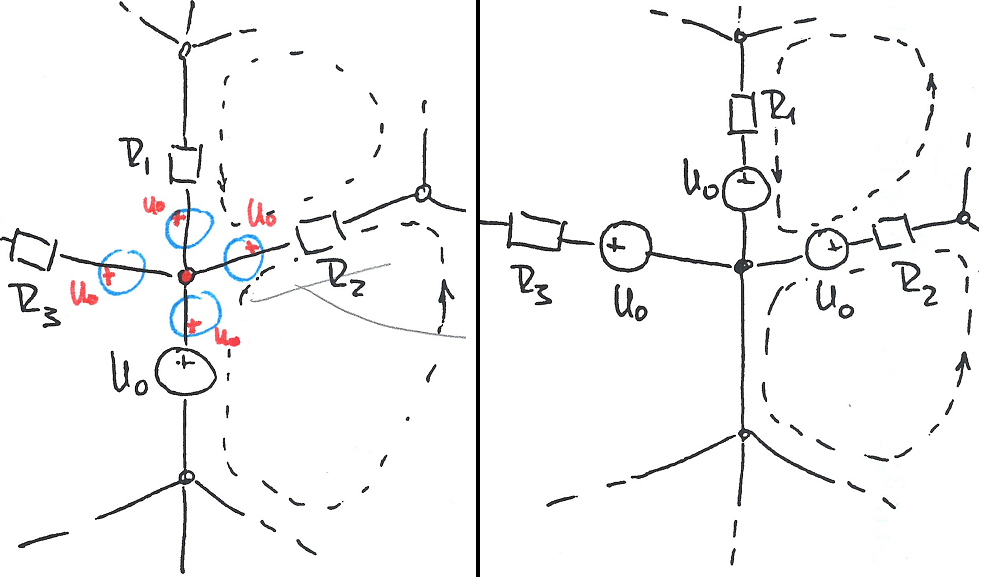
\includegraphics[width=0.4\textwidth]{pics/dcnet/UQuellenver}\\
Knotenpotential wird verändert $\rightarrow \varphi_B = \varphi_{B'} + U_o$
\end{center}
\begin{center}
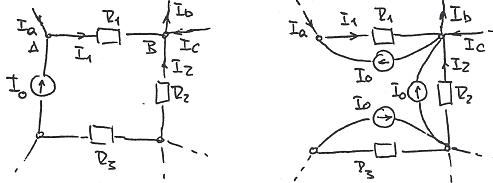
\includegraphics[width=0.5\textwidth]{pics/dcnet/IQuellenver}\\
Zweigstrom wird verändert $\rightarrow I_1 = j_1 + j_2 = I_0 + j_2$
\end{center}
\end{multicols}

